\section{Image Segmentation}
\subsection{Preliminaries}
\begin{itemize}
\item Separate the image into different parts, ie. regions or objects
\item It is a difficult but important task
\item Often a scene can be designed that the segmentation task is simplified
\item Segmentation is based on some property of the scene
\begin{itemize}
\item Intensity discontinuity
\item Intensity similarity
\item More Complex properties:
\begin{itemize}
\item Motion
\item Texture
\item Shape
\item Color
\item etc.
\end{itemize}
\end{itemize}
\end{itemize}

\subsection{Fundamentals}
\begin{enumerate}
\item $\bigcup\limits_{i=1}^{n}R_i=R$
\item $R_i$ is a connected set, $i=1,2,...,n$
\item $R_i\bigcap R_j = $ for all $i$ and $j, i\neq j$
\item $Q(R_i)=$TRUE for $i=1,2,...n$
\item $Q(R_i\bigcup R_j)=$FALSE for any adjacent Regions $R_i$ and $R_j$
\end{enumerate}
Focus on the intenxity values
\begin{itemize}
\item there are discontinuities, then a new region starts.
\item If the intensity does not vary much, then this is one region.
\end{itemize}

\subsection{Point, line and edge detection}
When the intensity changes abruptly in a local neighborhood, this indicates an edge. It can be a simple point or a line.\\
Abrupt local changes can be detected using derivatives.\\
First order derivative
\[
	\frac{\partial f}{\partial x} = f'(x)=f(x+1)-f(x)
\]
The second order derivative
\[
	\frac{\partial^2f}{\partial x^2}=\frac{\partial f'(x)}{\partial x}=f''(x)=f(x+1)+f(x-1)-2f(x)
\]
This can be calculated using a spatial filter.
\[
	\begin{matrix}
	w_1, w_2, w_3\\
	w_4, w_5, w_6\\
	w_7, w_8, w_9
	\end{matrix}
\]
\begin{itemize}
\item First order in y direction $w_6=1, w_5=-1$
\item First order in x direction $w_8=1, w_5=-1$
\item Second order in y direction $w_6=1, w_4=1, w_5=-2$
\item Second order in x direction $w_8=1, w_2=1, w_5=-2$
\end{itemize}
\subsubsection{Detection of Isolated Points}
The Laplacian combines the second derivatives in both spatial directions. This results in
\[
	\nabla^2f(x,y)=f(x+1,y)+f(x-1,y)+f(x,y+1)+f(x,y-1)-4f(x,y)
\]
It can be extended to also include the diagonal terms wich results in the following mask
\[
	\begin{matrix}
	 1 & 1 & 1\\
	 1 & -8 & 1\\
	 1 & 1 & 1
	\end{matrix}
\]
The Laplacian is isotropic with respect to $0^\circ, 45^\circ, 90^\circ and 135^\circ$. 

\subsubsection{Line Detection}
Often, a line of a known direction should be detected. We use special masks for that particular direction
\begin{figure}[h]
	\centering
	\begin{subfigure}[b]{0.2\textwidth}
		\centering
		\[
		\begin{array}{|c|c|c|}
			\hline
			-1 & -1 & -1\\
			\hline
			2 & 2 & 2\\
			\hline
			-1 & -1 & -1\\
			\hline
		\end{array}
		\]
		\caption{Horizontal}
	\end{subfigure}
	\begin{subfigure}[b]{0.2\textwidth}
		\centering
		\[
		\begin{array}{|c|c|c|}
			\hline
			2 & -1 & -1\\
			\hline
			-1 & 2 & -1\\
			\hline
			-1 & -1 & 2\\
			\hline
		\end{array}
		\]
		\caption{$+45^\circ$}
	\end{subfigure}
	\begin{subfigure}[b]{0.2\textwidth}
		\centering
		\[
		\begin{array}{|c|c|c|}
			\hline
			-1 & 2 & -1\\
			\hline
			-1 & 2 & -1\\
			\hline
			-1 & 2 & -1\\
			\hline
		\end{array}
		\]
		\caption{Vertical}
	\end{subfigure}
	\begin{subfigure}[b]{0.2\textwidth}
		\centering
		\[
		\begin{array}{|c|c|c|}
			\hline
			-1 & -1 & 2\\
			\hline
			-1 & 2 & -1\\
			\hline
			2 & -1 & -1\\
			\hline
		\end{array}
		\]
		\caption{$+45^\circ$}
	\end{subfigure}
	\caption{Line detection masks}
\end{figure}
%TODO Seite 20 Figure 10.10

\subsubsection{Edge localization}
The previously shown method generates edge points. The goal is to keep the ones which truly belong to an edge.\\
Since first order derivatives are helpful, a nice way of combining the two partial derivatives into one value is the magnitude of the gradient
\begin{equation}
	\nabla f = grad(f) = \left[\begin{array}{c} g_x \\ g_y \end{array}\right] =  \left[\displaystyle{\begin{array}{c} \frac{\partial f}{\partial x} \vspace{0.2cm}  \\ \frac{\partial f}{\partial y} \end{array}}\right] \notag
\end{equation}

The gradient (which is a vector) points into the direction of the greatest rate of change of f at the location (x,y)\\
The magnitude of the gradient vector is the value of the rate of change in that direction\\
Gradient operators:\\
\begin{figure}[h]
	\centering
	\begin{subfigure}[b]{0.2\textwidth}
		\centering
		\[
		\begin{array}{|c|c|c|}
			\hline
			-1 & -1 & -1\\
			\hline
			0 & 0 & 0\\
			\hline
			1 & 1 & 1\\
			\hline
		\end{array}
		\]
		\caption{Prewitt}
	\end{subfigure}
	\begin{subfigure}[b]{0.2\textwidth}
		\centering
		\[
		\begin{array}{|c|c|c|}
			\hline
			-1 & 0 & 1\\
			\hline
			-1 & 0 & 1\\
			\hline
			-1 & 0 & 1\\
			\hline
		\end{array}
		\]
		\caption{Prewitt}
	\end{subfigure}
	\begin{subfigure}[b]{0.2\textwidth}
		\centering
		\[
		\begin{array}{|c|c|c|}
			\hline
			-1 & -2 & -1\\
			\hline
			0 & 0 & 0\\
			\hline
			1 & 2 & 1\\
			\hline
		\end{array}
		\]
		\caption{Sobel}
	\end{subfigure}
	\begin{subfigure}[b]{0.2\textwidth}
		\centering
		\[
		\begin{array}{|c|c|c|}
			\hline
			-1 & 0 & 1\\
			\hline
			-2 & 0 & 2\\
			\hline
			-1 & 0 & 1\\
			\hline
		\end{array}
		\]
		\caption{Sobel}
	\end{subfigure}
	\caption{Prewitt and Sobel masks}
\end{figure}\\
After the gradient images have been calculated, often the magnitude of the gradient is required.
\[
	M(x,y) \approx |g_x|+|g_y|
\]
If the goal is to find the dominant edges, then smoothing the image before calculating the magnitude gradient image works well. Alternatively, the magnitude gradient image can also be thresholded such that only values above this value are considered edges (set to one). Everything else is set to 0.

\subsubsection{Marr-Hildreth edge detector}
New Idea: Edges exist on different scales. The edge detector needs to be tuned to the scale of the desired edge. Use a Gaussian filter (with space constant $\sigma$) and then take the Laplacian. The Gaussian filter is a low pass, wich blurs the image for large $\sigma$. This results in a Laplacian of Gaussian (LoG) filter.
\begin{figure}[h]
	\centering
	\begin{subfigure}[b]{0.45\textwidth}
		\centering
		\adjustbox{scale=0.5}{\usetikzlibrary{arrows}
\begin{tikzpicture}
	\draw[thick] (-6,0) -- (6,0);
	\draw[thick, -latex'] (0,-1) -- (0, 6.5) node[above] {$\nabla^2G$};
	
	\draw[latex-, thick] (-.85,0.10) -- ++(-1,1) -- ++(-1,0) node[left] {Zero Crossing};
	\draw[latex-, thick] (.85,0.10) -- ++(1,1) -- ++(1,0) node[right] {Zero Crossing};
	
	\draw[dashed] (-.85, 0) -- (-.85, -1.5);
	\draw[dashed] (.85, 0) -- (.85, -1.5);
	\draw (0,-1.3) node {$2\sqrt{2}\sigma$};
	\draw[-latex, thick] (-1.5,-1.3) --(-.85 , -1.3);
	\draw[-latex, thick] (1.5,-1.3) --(.85 , -1.3);	

	\draw[very thick] plot [smooth] coordinates {(-5,0) (-3.5,-0.05) (-1,-0.5) (0,6) (1,-0.5) (3.5,-0.05) (5,0)};
\end{tikzpicture}}
		\caption{Cross Section of the negative of the LoG, showing zero crossings}
	\end{subfigure}
	\begin{subfigure}[b]{0.45\textwidth}
		\centering
		\adjustbox{scale=0.75}{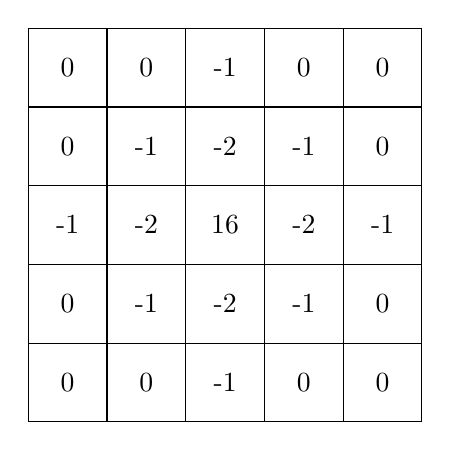
\begin{tikzpicture}

\foreach \x in {0,...,5} {
	\draw (\x,0) -- (\x,5);
	\draw (0,\x) -- (5,\x);
}

\foreach \x/\y in {0/0,1/0,0/1,3/0,4/0,4/1,0/3,0/4,1/4,3/4,4/4,4/3} {
	\node at  (\x+0.5,\y+0.5) {0};
}
\foreach \x/\y in {2/0,0/2,4/2,2/4,1/1,1/3,3/1,3/3} {
	\node at  (\x+0.5,\y+0.5) {-1};
}
\foreach \x/\y in {2/1,1/2,2/3,3/2} {
	\node at  (\x+0.5,\y+0.5) {-2};
}

\node at (2.5,2.5) {16};

\end{tikzpicture}}
		\caption{5x5 mask approximation. The negative of this mask would be used in practicej}
	\end{subfigure}
	\caption{Marr-Hildreth}
\end{figure}

\textbf{Summary of the Marr-Hildreth edge detection:}
\begin{enumerate}
\item Filter the input image with an $n x n$ Gaussian lowpass filter $G(x,y)=e^{-\frac{x^2+y^2}{2\sigma^2}}$
\item Compute the Laplacian of the image resulting from Step 1. $\nabla ^2[G(x,y) \star f(x,y)]$
\item Find the zero crossing of the image from Step 2.
\end{enumerate}
\textbf{Size of the discrete LoG filter}
Rule of thumb: nxn LoG filter should have the smallest odd integer n greater than or equal to $6\sigma$.\\
\textbf{How to find the zero crossings?}
A zero-crossing exists, if at least one opposing pixelpair has a sign difference.
%TODO Matrix edge detection
%*rx 
%o o
%xr*
%zwei paare davon müssen ein vorzeichen ändern

\subsubsection{Canny edge detector}
More complex, more powerful. The derivation is powerful, the implementation easy. Canny uses the gradient angle image and the linking of weak with strong edges.\\
Smooth the image and then find the gradient vector magnitude and direction:
\begin{align*}
G(x,y) = e^{-\frac{x^2+y^2}{2\sigma^2}}\\
f_s(x,y)=G(x,y)\star f(x,y)\\
M(x,y) = \sqrt{g_x^2+g_y^2}\\
\alpha(x,y) = tan^{-1}\left[\frac{g_y}{g_x}\right]\\
\end{align*}
The first new idea is, to thin the edges, using the gradient directional information. This is called nonmaxima suppression.\\
%TODO ?
We are looking for the maxima of the gradient magnitude along the gradient direction. $g_N(x,y)$ is the nonmaxima-suppressed image, the gradient magnitude image where the wide ridges have been thinned since the middle value is only kept when it is the maxima within a 3x3 neighborhood along the gradient direction.\\
This image is thresholded to find the significant edges and remove the noise.

\begin{itemize}
\item $T_H$ high threshold. The values above this are almost certainly true edges
\item $T_L$ low threshold. The values above this are likely to be edges. If they are 8-connected to a edge in $g_{NH}(x,y)$, they are also an edge.
\end{itemize}
%TODO Seite 50 summary canny

\subsubsection{Edge linking and boundary detection}
Three schemes to link edges:\\
\textbf{Local processing}\\
For every point at a location the gradient vector magnitude and angle are compared with the magnitude and angle of points in a neighborhood. If these are similar, they belong to the same boundary. This can be indicated by giving them the same color and/or gray value.\\
A much simpler scheme can be used if the linking follows certain directions and the maximum gap size is roughly known.\\
%TODO enumerate seite 55
\textbf{Regional processing}\\
If the location of a boundary is roughly known, it is possible to use the detected edge points as indicators for the suspected boundary.
\begin{enumerate}
\item Let P be a sequence of ordered, destinct, 1-valued points of a binary image. Specify two starting points, A and B. these are two starting vertices of the polygon.
\item Specify a threshold T, and two empty stacks, OPEN and CLOSED.
\item If the points in P correspond to a closed curve, put A into OPEN and put B into OPEN and CLOSED.
\item Compute the parameters of the line passing from the last vertex in CLOSED to the last vertex in OPEN.
\item Compute the distances from the line in Step 4 to all the points in P whose sequence places them between the vertices from Step 4. Select the point, $V_{max}$, with the maximum distance $D_{max}$ (ties are resolved arbitrarily)
\item If $D_{max}$, place $V_{max}$ at the end of the OPEN stack as a new vertex. Go to Step 4.
\item Else, remove the last vertex from Open and insert it as the last vertex of CLOSED.
\item If OPEN is not empty, go to Step 4.
\item Else, exit. The vertices in CLOSED are the vertices of the polygonal fit to the points in P.
\end{enumerate}
\begin{figure}[h]
	\centering
	\adjustbox{scale=0.5}{\usetikzlibrary{calc}
\begin{tikzpicture}[dot/.style={circle,inner sep=1pt, fill, name=#1}]

\begin{scope}[shift={(-5.5,1)}]
\node [dot=A] at (-2,-1.4) {};
\node [dot=B] at (-2.4,0.4) {};
\node [dot=C] at (1.2,-2.2) {};
\node [dot=D] at (2.2,-1.4) {};
\node [dot=E] at (2.6,-0.2) {};
\node [dot=F] at (2.4,0.8) {};
\node [dot=G] at (-1.6,1.8) {};
\node [dot=H] at (-2.2,1.2) {};
\node [dot=I] at (-2.4,-0.6) {};
\node [dot=J] at (2,1.6) {};
\node [dot=K] at (1.2,2) {};
\node [dot=L] at (0.4,2.4) {};
\node [dot=M] at (-0.8,2.2) {};
\draw[thick] (A) -- (C);
\draw[thick, dashed] ($(A)!(L)!(C)$) -- (L);
\end{scope}

\begin{scope}[shift={(0.9,1)}]
\node [dot=A] at (-2,-1.4) {};
\node [dot=B] at (-2.4,0.4) {};
\node [dot=C] at (1.2,-2.2) {};
\node [dot=D] at (2.2,-1.4) {};
\node [dot=E] at (2.6,-0.2) {};
\node [dot=F] at (2.4,0.8) {};
\node [dot=G] at (-1.6,1.8) {};
\node [dot=H] at (-2.2,1.2) {};
\node [dot=I] at (-2.4,-0.6) {};
\node [dot=J] at (2,1.6) {};
\node [dot=K] at (1.2,2) {};
\node [dot=L] at (0.4,2.4) {};
\node [dot=M] at (-0.8,2.2) {};
\draw[thick] (A) -- (L) -- (C);
\draw[thick, dashed] ($(A)!(H)!(L)$) -- (H);
\draw[thick, dashed] ($(L)!(F)!(C)$) -- (F);
\end{scope}

\begin{scope}[shift={(-5.5,-5)}]
\node [dot=A] at (-2,-1.4) {};
\node [dot=B] at (-2.4,0.4) {};
\node [dot=C] at (1.2,-2.2) {};
\node [dot=D] at (2.2,-1.4) {};
\node [dot=E] at (2.6,-0.2) {};
\node [dot=F] at (2.4,0.8) {};
\node [dot=G] at (-1.6,1.8) {};
\node [dot=H] at (-2.2,1.2) {};
\node [dot=I] at (-2.4,-0.6) {};
\node [dot=J] at (2,1.6) {};
\node [dot=K] at (1.2,2) {};
\node [dot=L] at (0.4,2.4) {};
\node [dot=M] at (-0.8,2.2) {};
\draw[thick] (A) -- (H) -- (L) -- (F) -- (C);
\draw[thick, dashed] ($(A)!(I)!(H)$) -- (I);
\draw[thick, dashed] ($(L)!(M)!(H)$) -- (M);
\draw[thick, dashed] ($(L)!(J)!(F)$) -- (J);
\draw[thick, dashed] ($(F)!(D)!(C)$) -- (D);
\end{scope}

\begin{scope}[shift={(0.9,-5)}]
\node [dot=A] at (-2,-1.4) {};
\node [dot=B] at (-2.4,0.4) {};
\node [dot=C] at (1.2,-2.2) {};
\node [dot=D] at (2.2,-1.4) {};
\node [dot=E] at (2.6,-0.2) {};
\node [dot=F] at (2.4,0.8) {};
\node [dot=G] at (-1.6,1.8) {};
\node [dot=H] at (-2.2,1.2) {};
\node [dot=I] at (-2.4,-0.6) {};
\node [dot=J] at (2,1.6) {};
\node [dot=K] at (1.2,2) {};
\node [dot=L] at (0.4,2.4) {};
\node [dot=M] at (-0.8,2.2) {};
\draw[thick] (A) -- (I) -- (H) -- (M) -- (L) -- (J) -- (F)-- (D) -- (C);
\end{scope}

\end{tikzpicture}}
	\caption{Regional Processing}
\end{figure}
\textbf{Global processing}\\
\subsubsection{Hough transform}
\begin{itemize}
%TODO Figure 10.31 Seite 63 und Bild Normale Seite 64
\item Each point in the xy plane belongs to infinetly many lines $y_i=ax_i+b$
\item If we interpret this line equation differently, then $b=-x_ia+y_i$ represent for each point in the xy plane a line in the ab plane
\item For each point in the xy plane, a line can be drawn in the ab plane and the principal lines in the xy plane can be found by the points with the most intersections in the ab plane
\item Vertical lines require an infinite a, this does not work. Use the line normal as representation. A point in the xy plane does not result in a simple straight line in the parameter space ($\theta\rho$). The curve $\rho = f(\theta)$ is now a sinusoidal
\item Practical scheme
\begin{itemize}
\item For every $\theta_q$ in the $\rho\theta$ plane
\item Calculate $\rho = f(\theta)$ and quantize it into $\rho_q$
\item Increase the cell in the $\rho\theta$ plane at location ($\rho_q, \theta_q$) by one
\item end
\end{itemize}
\end{itemize}

\subsection{Thresholding}
\subsubsection{Basic global thresholding}
\begin{equation}
g(x,y)=\begin{cases}1 \qquad \text{if } f(x,y) > T \\0 \qquad  \text{if } f(x,y) \leq T \end{cases} \label{thresholdingBasic}
\end{equation}

\begin{enumerate}
\item Select an initial estimate for the global threshold, T
\item Segment the image using T in Gleichung(\ref{thresholdingBasic}). This will produce two groups of pixels: $G_1$ consisting of all pixels with intensity values $> T$, and $G_2$ consisting of pixels with values $\leq T$
\item Compute the average (mean) intensity values $m_1$ and $m_2$ for the pixels in $G_1$ and $G_2$, repsectively
\item Compute a new threshold value: \begin{equation}
T=\frac{1}{2}(m_1+m_2)\notag
\end{equation} 
\item Repeat Steps 2 through 4 until the difference betwenn values of $T$ in successive iterations is smaller than a predefined paramter $\Delta T$
\end{enumerate}
\subsubsection{Optimum global thresholding using Otsu’s Method}

Two different variances are important
\begin{itemize}
\item Within-class variance
\item Between-class variance
\end{itemize}
\begin{eqnarray}
\sigma_W^2 = P_1\sigma_1^2+P_2\sigma_2^2 
& & \sigma_W \text{ Within-class variance} \notag \\
\sigma_B^2 = P_1(m_1-m_G)^2+P_2(m_2-m_G)^2
& & \sigma_B \text{ Between-class variance} \notag \\
\sum_{i=0}^{L-1} p_i = 1 
& & \notag \\
m_G=\sum_{i=0}^{L-1} i \ p_i 
& & m_G: \text{ global mean}  \notag \\
\sigma_G^2 = \sum_{i=0}^{L-1} (i-m_G)^2 p_i
& & \sigma_G \text{global variance} \notag \\
P_1(k) =\sum_{i=0}^{k} p_i
& &  P_1: \text{ probability of the background}   \notag \\
P_2(k)=\sum_{i=k+1}^{L-1}1-P_1(k)
& & P_2: \text{ probability of the object} \notag \\
m_1(k)=\frac{1}{P_1(k)}\sum_{i=0}^{k} i \ p_i
& &  m_1: \text{ mean intensity of the background}  \notag \\
m_2(k)=\frac{1}{P_2(k)}\sum_{i=k+1}^{L-1} i \ p_i 
& &  m_2: \text{ mean intensity of the object}  \notag \\
\sigma_B^2 = P_1(m_1-m_G)^2+P_2(m_2-m_G)^2 & &  \text{Using algebra to change the form} \notag \\
=P_1 P_2 (m_1-m_2)^2 = \frac{(m_G P_1 - m)^2}{P_1(1-P_1)} & & \notag \\
\sigma_B^2(K*)=\max\limits_{0\leq k \leq L-1} \sigma_B^2(K)
& & \text{Optimum of k for maximizing is } k* \notag \\
\eta(k)=\frac{\sigma_B^2(k)}{\sigma_G^2}
& & 0 \leq  \eta(k*)\leq 1 \notag
\end{eqnarray}

\subsubsection{Variable Thresholding}
\textbf{Image Partitioning}\\
The simplest approach is to partition a given image into non overlapping regions and then use Otsu's method on smaller regions.\\
\textbf{Based on local image properties}\\
A threshold is computed for each point. The threshold depends on some property of a local neighborhood. Common properties are the mean and standard deviation for each pixel.
An even more powerful scheme can be built, if the 1 or 0 decision is based on some logical condition.\\

\subsection{Region based segmentation}
The goal is to segment the image into regions directly, not using abrupt changes or thresholding.
\subsubsection{Region growing}
\begin{enumerate}
\item Find all connected components in $S(x,y)$ and erode each connected component to one pixel; label all such pixels found as 1. All other pixels in S are labeled 0.
\item Form an image $f_Q$ such that, at a pair of coordinates...
%TODO Folie 104 Nr. 1 bis 4 schreiben
\end{enumerate}
\subsubsection{Region splitting and merging}
The image is subdivided initially into a set of arbitrary disjoint regions and then the regions are merge and or split in an attempt to improve the segmentation.\\
A common scheme to split images is a quadtree.\\
%TODO Seite 107 Schritt 1 bis 3
%TODO Seite 107 Bild a und b
\subsubsection{Segmentation using morphological watersheds}
The basic idea is to think of images as 3D landscapes. There are three kinds of points:
\begin{itemize}
\item Points belonging to a regional minimum.
\item Points, where water would flow. These are called catchment basin.
\item Points, where water would be equally likely to fall to more than one such minimum. These are called watershed.
\end{itemize}
Basic idea:
\begin{itemize}
\item In each basin a hole is punched
\item The topological image is pushed into a full bathtub. The water rises uniformly in the different basing
\item As soon as the water in different basins want to merge, a dam is build
\item At the end only the dams are left. These are the watershed lines wich are connected boundaries segmenting the image into different regions.
\end{itemize}
\textbf{Watershed segmentation algorithm}
\begin{itemize}
\item $T[n]$ is the set of coordinates flooded $T[n] = {(s,t)|g(s,t)<n}$
\item The flooding goes in integers from $n=min+1$ to $n=max+1$
\item The algorithm starts with $C[min+1]=T[min+1]$. This leads to $C_{min+1}(M_i)$ for every minimum. $C[n]=\bigcup\limits_{i=1}^{R}C_n(M_i)$
\item Now $C[n]$ is created from $C[n-1]$
\begin{enumerate}
\item Was a new basin discovered?
\item Did the basins simply expand?
\item Did two basins merge?
\end{enumerate}
%TODO Algorithm Seite 114 und 115
%TODO dam building algo Seite 112
\end{itemize}
\subsubsection{The use of motion in segmentation}
%TODO Seiten 117, 118, 119